
\hypertarget{multiple-control-variables}{}
\section{Multiple Control Variables and Modularity}\label{sec:multiple-control-variables}

We now consider problems with multiple control variables.  Section~\ref{subsec:JointProblem} presents the joint consumption-and-portfolio optimization as a canonical example: we derive the simultaneous first-order conditions and show that direct numerical solution of the multidimensional problem is computationally expensive---but that decomposing it into a sequence of single-control problems is much faster.  Section~\ref{subsec:stageswithin} develops the stage-based machinery for such decompositions, building on the modular notation from section~\ref{sec:notation}: the discounting {\stg} (\StgName{disc}), the standalone portfolio optimization (section~\ref{subsec:MCTheory}), and the general-purpose \StgName{portable} returns {\stg} that unifies portfolio choice and shock realization.  Section~\ref{subsubsec:three-period-types} combines these building blocks into three canonical {\interval} types.

\hypertarget{joint-optimization-problem}{}
\subsection{The Joint Optimization Problem}\label{subsec:JointProblem}\label{subsec:MCApplication}

Our canonical example of a multi-control problem is the case where the agent has both a consumption choice and a decision about $\Shr$ (archaic Greek \href{https://en.wikipedia.org/wiki/Stigma_(ligature)}{stigma}): the share of assets in the risky asset.  Given a risky-asset return factor $\Risky$ and a riskless return factor $\Rfree$, the realized portfolio return is
\hypertarget{eq-Rport}{}
\begin{equation}\begin{gathered}\begin{aligned}
      \Rport(\Shr) &= \Rfree+(\Risky-\Rfree)\Shr \label{eq:Rport}.
    \end{aligned}\end{gathered}\end{equation}
Written as a single combined decision (substituting the budget constraint):
\hypertarget{eq-Bellmanundated}{}
\begin{equation}\begin{gathered}\begin{aligned}
  \vFunc_{\prdt}(\mNrm)  & = \max_{\{\cFunc,\Shr\}} ~~  \uFunc(\cNrm) + \ExDcsn[\DiscFac \vFunc_{\prdt+1}(
              \overbrace{(\mNrm-\cNrm)\Rport(\Shr) + {\tranShkEmp}}^{\mNrm_{t+1}}
              )] \label{eq:Bellmanundated}
\UnifiedNote{𝒱(m) = max_{c,ς} u(c) + β·E[𝒱₊(gᵥₑ(m, c, ς))] [combined decision value; no stage decomposition — motivates splitting into sequential stages]}
    \end{aligned}\end{gathered}\end{equation}
Whether the stochastic variables $\Risky$ and $\tranShkEmp$ are revealed at the end of the current {\interval} or the start of the next does not affect this equation.  The first-order conditions for this joint problem are:
\begin{equation}\begin{gathered}\begin{aligned}
      \uFunc^{\partial}(\cNrm)  & = \vCntn^{\partial a}(\mNrm-\cNrm,\Shr)
      \\      0  & = \vCntn^{\partial \Shr}(\mNrm-\cNrm,\Shr) \label{eq:FOCjoint}
\UnifiedNote{Simultaneous FOCs: u'(c) = ℰ^{\partial}ₐ(m−c, ς) and 0 = ℰ^{\partial}_ς(m−c, ς) [joint optimization; contrast with sequential stage decomposition]}
    \end{aligned}\end{gathered}\end{equation}

Direct simultaneous solution of these two conditions is computationally expensive; the remainder of this section develops modular {\stg}-based machinery that decomposes the problem into a sequence of simpler single-control optimizations.

\begin{comment}
\paragraph{Numerical solution of the joint problem.}\label{subsec:MCApplication}

The continuation value $\vCntn(a,\Shr)$ incorporates the discount factor $\DiscFac$; hence $\DiscFac$ appears explicitly when the expectation is expanded to the next {\interval}'s consumption function.

In specifying the stochastic process for $\Risky_{\prdt+1}$, we follow the common practice of assuming that returns are lognormally distributed, $\log \Risky \sim \Nrml(\eprem+\rfree-\sigma^{2}_{\risky}/2,\sigma^{2}_{\risky})$ where $\eprem$ is the equity premium over the thin returns $\rfree$ available on the riskless asset.\footnote{This guarantees that $\Ex[\Risky] = \pmb{\varphi}/\Rfree$ is invariant to the choice of $\sigma^{2}_{\risky}$; see \handoutM{LogELogNorm}.}

As with labor income uncertainty, it is necessary to discretize the rate-of-return risk in order to have a problem that is soluble in a reasonable amount of time.  We follow the same procedure as for labor income uncertainty, generating a set of $n_{\risky}$ equiprobable shocks to the rate of return; in a slight abuse of notation, we will designate the portfolio-weighted return (contingent on the chosen portfolio share in equity, and potentially contingent on any other aspect of the consumer's problem) simply as $\Rport_{i,j}$ (where dependence on $i$ is allowed to permit the possibility of nonzero correlation between the return on the risky asset and the $\tranShkEmp$ shock to labor income (for example, in recessions the stock market falls and labor income also declines)).

The direct expressions for the derivatives of $\vCntn$ are
\begin{equation}\begin{gathered}\begin{aligned}
      \vCntn^{\partial a}(a_{\prdt},\Shr_{\prdt})  & = \DiscFac \left(\frac{1}{n_{\risky} n_{\tranShkEmp}}\right)\sum_{i=1}^{n_{\tranShkEmp}}\sum_{j=1}^{n_{\risky} }\Rport_{i,j} \left(\cFunc_{\prdt+1}(\Rport_{i,j}a_{\prdt}+\tranShkEmp_{i})\right)^{-\CRRA}
      \\      \vCntn^{\partial \Shr}(a_{\prdt},\Shr_{\prdt})  & = \DiscFac \left(\frac{1}{n_{\risky} n_{\tranShkEmp}}\right)\sum_{i=1}^{n_{\tranShkEmp}}\sum_{j=1}^{n_{\risky} }(\Risky_{i,j}-\Rfree)\left(\cFunc_{\prdt+1}(\Rport_{i,j}a_{\prdt}+\tranShkEmp_{i})\right)^{-\CRRA}a_{\prdt}.
\UnifiedNote{ℰ^{\partial}ₐ(a, ς) and ℰ^{\partial}_ς(a, ς) [discretized continuation-value partial derivatives over (a, ς) grid]}
    \end{aligned}\end{gathered}\end{equation}

Writing these equations out explicitly makes a problem very apparent: For every different combination of $\{{a}_{\prdt},\Shr_{\prdt}\}$ that the routine wishes to consider, it must perform two double-summations of $n_{\risky} \times n_{\tranShkEmp}$ terms.  Once again, there is an inefficiency if it must perform these same calculations many times for the same or nearby values of $\{{a}_{\prdt},\Shr_{\prdt}\}$, and again the solution is to construct an approximation to the (inverses of the) derivatives of the $\vCntn$ function.

Assume we have the approximations $\Aprx{\vFunc}_{\Cntn}^{\partial a}$ and $\Aprx{\vFunc}_{\Cntn}^{\partial \Shr}$ in hand and want to proceed.  Given the formulation in \eqref{eq:Bellmanundated}, nonlinear equation solvers can find the solution to a set of simultaneous equations.  Thus we could ask one to solve
\begin{equation}\begin{gathered}\begin{aligned}
      \cNrm_{\prdt}^{-\CRRA}  & = \Aprx{\vFunc}^{\partial a}_{{\cntn}(\prdt)}(\mNrm_{\prdt}-\cNrm_{\prdt},\Shr_{\prdt}) %\label{eq:FOCwrtcMultContr}
      \\      0  & = \Aprx{\vFunc}^{\partial \Shr}_{{\cntn}(\prdt)}(\mNrm_{\prdt}-\cNrm_{\prdt},\Shr_{\prdt}) \label{eq:FOCwrtw}
    \end{aligned}\end{gathered}\end{equation}
simultaneously for $\cNrm$ and $\Shr$ at the set of potential $\mNrm_{\prdt}$ values defined in {\mVec}. However, as noted above, multidimensional constrained
maximization problems are difficult and sometimes quite slow to
solve.
\end{comment}

\begin{comment}
\paragraph{A better way.}

There is a better way.  Define the problem

\begin{equation}\begin{gathered}\begin{aligned}
      \Opt{\vFunc}_{{\cntn}(\prdt)}(a_{\prdt})  & = \max_{\Shr_{\prdt}} ~~  \vCntn(a_{\prdt},\Shr_{\prdt})
      \\      & \text{s.t.} \nonumber
      \\      0 \leq & \Shr_{\prdt} \leq 1
\UnifiedNote{ℰ̃(a) = max_ς ℰ(a, ς) s.t. 0 ≤ ς ≤ 1 [reduce to single-control by optimizing over ς]}
    \end{aligned}\end{gathered}\end{equation}
where the tilde over $\Opt{\vFunc}(a)$ indicates that this is the $\vFunc$ that has been optimized with respect to all of the arguments other than the one still present ($a_{\prdt}$).  We solve this problem for the set of gridpoints in \code{aVec} and use the results to construct the interpolating function $\Aprx{\Opt{\vFunc}}_{\prdt}^{\partial}(a_{\prdt})$.\footnote{A faster solution could be obtained by, for each element in \code{aVec}, computing $\vCntn^{\partial \Shr}(m_{\prdt}-c_{\prdt},\Shr)$ of a grid of values of $\Shr$, and then using an approximating interpolating function (rather than the full expectation) in the \texttt{FindRoot} command.  The associated speed improvement is fairly modest, however, so this route was not pursued.}  With this function in hand, we can use the first order condition from the single-control problem
\begin{equation*}\begin{gathered}\begin{aligned}
      c_{\prdt}^{-\CRRA}  & = \Aprx{\Opt{\vFunc}}_{\prdt}^{\partial}(m_{\prdt}-c_{\prdt})
    \end{aligned}\end{gathered}\end{equation*}
to solve for the optimal level of consumption as a function of $m_{\prdt}$ using the endogenous gridpoints method described above.  Thus we have transformed the multidimensional optimization problem into a sequence of two simple optimization problems.

Note the parallel between this trick and the fundamental insight of dynamic programming: Dynamic programming techniques transform a multi-period (or infinite-period) optimization problem into a sequence of two-period optimization problems which are individually much easier to solve; we have done the same thing here, but with multiple dimensions of controls rather than multiple periods.

The remainder of this section develops a general framework, building on the modular notation from section~\ref{sec:notation}, that formalizes this sequential decomposition into reusable single-control {\stgs}.
\end{comment}

\hypertarget{stages-within-a-period}{}
\subsection{Decomposing Into Modular Stages}\label{subsec:stageswithin}

The single-{\stg}-per-{\interval} formulation from \ifthenelse{\boolean{shortVersion}}{sections~\ref{sec:the-problem}--\ref{sec:the-usual-theory}}{sections~\ref{sec:the-problem}--\ref{sec:solving-the-next}} is equivalent to a sequence of simpler {\stgs}, each with a single job.  We decompose it in that way so that adding portfolio choice later requires no change to the consumption-{\stg} code---only the stage list and the {\Cnct}s between {\stgs} change (see section~\ref{sec:notation}).  The decomposition yields the same value functions, consumption function, and Euler equation.

\hypertarget{disc-stage}{}
\subsubsection{The Discounting Stage (\StgName{disc})}\label{subsubsec:disc-stage}

The simplest decomposition isolates discounting into a standalone {\stg} that applies for the entire period.  We call it the \StgName{disc} {\stg} (control-name $\DiscFac$).  From equation~\eqref{eq:trns-single-prd}, $\vEndPrd \leftassign \DiscFac \vBegPrdNxt$; the factor $\DiscFac$ was implicitly inside the backward builder $\BkBldrPrd$ that created $\vCntn$.  Instead, henceforth at the end of every {\interval},  we put the stub \StgName{disc} {\stg} which has no choice, no shocks, and a trivial decision value function $\vDcsn = \DiscFac \cdot \vCntn$, and we set the discount factor to 1 for every prior stage in the period (leaving all the discounting to the \StgName{disc} stage).\footnote{Equations in sections~\ref{sec:the-problem}--\ref{sec:the-usual-theory}, which predate the modular decomposition, show $\DiscFac$ inside the continuation value of the consumption problem (e.g., \eqref{eq:vNormed}).  That formulation is equivalent: the $\DiscFac$ that appears there is the same discount factor, housed inside a composite continuation value rather than in a separate {\stg}.  The modular decomposition separates what those equations combine.}

\begin{table}[h]\caption{Discounting {\Stg} ($\DiscFac$) {\Prchs}}\label{tab:prchs-disc}
\newsavebox{\disctablebox}%
\begin{center}
    \savebox{\disctablebox}{\begin{tabular}{r|c|c|c|l}
      {\Prch}         & Indicator        & State    & value functions                             & Explanation    \\ \hline
      {\Arrival}      & $ \arvl $        & $\bullet$      & $\vArvl = \vDcsn$          & no shocks    \\
      {\Decision}(s)  & $\sim$           & $\bullet$      & $\vDcsn = \DiscFac \vCntn$ & apply $\DiscFac$ \\ 
      {\Continuation} & $ \cntn $        & $\bullet$      & $\vCntn$                                   & value at exit \\ \hline
    \end{tabular}}%
    \usebox{\disctablebox}

    \parbox{\wd\disctablebox}{\footnotesize n.b.: $\bullet$ is a generic passthrough state whose type (k-type or m-type) is inherited from the predecessor {\stg}'s {\Continuation} state.  For example, when \StgName{disc} follows \StgName{cons-noshocks}, $\bullet$ stands for $\aNrm$ (k-type); when it follows \StgName{portable}, $\bullet$ stands for $\check{\mNrm}$ (m-type).}
  \end{center}
  \end{table}

%  Now we specify the consumption {\stg} to have $\DiscFac = 1$; the \StgName{disc} {\stg} receives $\aNrm$ and the backward builder $\BkBldrPrd$ constructs $\vFunc_{\DiscFac,\dcsn} = \DiscFac \cdot \vFunc_{\DiscFac,\cntn}(\aNrm)$ and $\vArvl=\vDcsn$.

  The two-{\stg} {\interval} has stage list $[\StgName{cons-with-shocks}, \StgName{disc}]$ (more compactly, $[\cFunc, \DiscFac]$).  The convention that every non-\StgName{disc} {\stg} is undiscounted and every {\interval} ends with \StgName{disc} will mean we do not have to rearrange discounting as we rearrange stages within the period.

\hypertarget{standalone-portfolio-problem}{}
\subsubsection{The Standalone Portfolio Problem}\label{subsec:MCTheory}

Consider the standalone problem of an `investor' choosing the portfolio share $\Shr$.  The state variable at the start is $\kNrm$ (capital available for investment); the {\Decision} chooses $\Shr$; stochastic shocks ($\Risky$, $\tranShkEmp$) are then realized, yielding the {\Continuation} state $\check{\mNrm} = \Rport(\Shr)\kNrm + \tranShkEmp$.  The portfolio share must be chosen \textit{before} the return shock $\Risky$ is realized.  We write $\check{\mNrm}$ rather than $\mNrm$ for the post-shock state because a strict rule of our framework is the prohibition of multiple timings of a given variable within a period.  Note that $\check{\mNrm}$ is m-type (market resources after shocks), matching $\mNrm$; the $\check{}$ decoration distinguishes the two timings while preserving the type (see section~\ref{subsec:transitions}).

The first-order condition with respect to $\Shr$ is:
\hypertarget{eq-FOCport}{}
\begin{equation}\begin{gathered}\begin{aligned}
  0 & = \Ex_{\dcsn}\left[
      (\Risky-\Rfree)\vFunc^{\dcheckm}_{\cntn}(\check{\mNrm})
      \right] \label{eq:FOCport}
\UnifiedNote{0 = E_dcsn[(R̃ − R) · ℰ^{\partial}_port(m̌)] [portfolio stage FOC; optimality condition for ς in 𝒱_port]}
\end{aligned}\end{gathered}\end{equation}
where $\vFunc^{\dcheckm}_{\cntn}$ denotes the derivative of the continuation value function with respect to $\check{\mNrm}$.

The {\Decision} equation yields the portfolio share function:
  \begin{equation}\begin{gathered}\begin{aligned}
    \Shr(\kNrm)  = & \argmax_{\Shr}~~ \Ex_{\dcsn}
                    \left[\vFunc_{\cntn}
                    \left(
%                    \overbrace{
              (\Rfree+(\Risky-\Rfree)\Shr)\kNrm + \tranShkEmp
              %}^{\check{\mNrm}}
                    \right)
                    \right] \label{eq:shrDecision},
\UnifiedNote{𝒱_port decision: ς*(k) = argmax_ς E_ζ[ℰ_port(gᵥₑ(k, ς, ζ))] where gᵥₑ: (k, ς, ζ) → m̌ = k(ςR̃ + (1−ς)R) + θ, ζ = (R̃, θ)}
         \end{aligned}\end{gathered}\end{equation}

\hypertarget{portable}{}
\subsubsection{The \StgName{portable} Stage}\label{subsubsec:portable}

The portfolio optimization problem above can be generalized into a single configurable \textit{returns-and-shocks} {\stg} by making the portfolio share an \textit{optional parameter} rather than a control variable that must always be optimized.  We call this the \StgName{portable} {\stg} (``\textit{port}folio-\textit{able}''): it is ``able'' to perform portfolio optimization or not, depending on a parameter $\bar{\Shr}$.

The {\stg}'s {\Arrival} state includes the investable capital $\kNrm$ and an optional portfolio share $\bar{\Shr} \in [0,1] \cup \{\bot\}$, where $\bot$ means ``absent---optimize.''  The behavior of the {\stg} depends on $\bar{\Shr}$:
\begin{itemize}
\item \textbf{Optimize mode} ($\bar{\Shr} = \bot$): The {\stg} solves the portfolio optimization problem from section~\ref{subsec:MCTheory}, choosing $\Shr$ optimally via~\eqref{eq:shrDecision} with first-order condition~\eqref{eq:FOCport}.
\item \textbf{Fixed-share mode} ($\bar{\Shr} \in [0,1]$): The portfolio share is prescribed; no optimization occurs.  The value function is $\vArvl(\kNrm, \bar{\Shr}) = \Ex_{\arvl}[\vCntn(\Rport(\bar{\Shr})\kNrm + \tranShkEmp)]$.
\item \textbf{No-risky-investment mode} ($\bar{\Shr} = 0$): A special case of fixed-share mode.  All assets earn the riskless return: $\check{\mNrm} = \Rfree \kNrm + \tranShkEmp$.  The risky return $\Risky$ is irrelevant.  The value function reduces to $\vArvl(\kNrm, 0) = \Ex_{\arvl}[\vCntn(\Rfree \kNrm + \tranShkEmp)]$.
\end{itemize}

\noindent The {\prchs} of this {\stg} are:

\begin{table}[h]\caption{\StgName{portable} {\Stg} {\Prchs}}\label{tab:prchs-portable}
\begin{center}
    \begin{tabular}{r|c|c|c|l}
      {\Prch}         & Indicator        & State              & value functions                                     & Explanation    \\ \hline
      {\Arrival}      & $ \arvl $        & $(\kNrm, \bar{\Shr})$   & $\vArvl = \vDcsn$                                    & no pre-decision shocks \\
      {\Decision}(s)  & $\sim$           & $(\kNrm, \bar{\Shr})$   & depends on $\bar{\Shr}$ (see above)                  & choose $\Shr$ or use $\bar{\Shr}$ \\
      {\Continuation} & $ \cntn $        & $\check{\mNrm}$          & $\vCntn$                              & post-shock value \\ \hline
    \end{tabular}
  \end{center}
  \end{table}

\noindent When $\bar{\Shr} = \bot$, the {\Decision} value function is $\vDcsn = \max_{\Shr} \Ex_{\dcsn}[\vCntn]$.  When $\bar{\Shr} \in [0,1]$, it is $\vDcsn = \Ex[\vCntn]$ with $\Shr$ fixed at $\bar{\Shr}$.

\hypertarget{argument-notation}{}
\paragraph{Argument notation.}  When a stage can be constructed with a fixed parameter, we write the value of that argument in parentheses.  Thus $\Shr(0)$ denotes the \StgName{portable} stage with $\bar{\Shr}=0$ (the \StgName{shocks-only} configuration described below), and $\Shr(\bot)$ denotes \StgName{portable} in optimize mode.

\hypertarget{shocks-only-decomposition}{}
\subsubsection{Separating Shocks from Choices}\label{subsubsec:shocks-cons-decomp}

The \StgName{cons-with-shocks} {\stg} in section~\ref{subsec:prchs} combines the $\kNrm \to \mNrm$ shock realization and the $\mNrm \to \aNrm$ consumption decision.  We split these into two {\stgs}.

\paragraph{The \StgName{shocks-only} stage (\StgName{portable} with $\bar{\Shr}=0$).}  Calling the \StgName{portable} {\stg} with $\bar{\Shr}=0$ produces a {\stg} whose only function is to draw the shocks.  We call this configuration \StgName{shocks-only}.  It handles the transition from capital $\kNrm$ to (post-shock) market resources $\check{\mNrm}$: with $\Shr = 0$, the transition is $\check{\mNrm} = \RNrmByG \kNrm + \tranShkEmp$---precisely the $\kNrm \to \check{\mNrm}$ mapping from the original problem (the next stage receives this as $\mNrm$).  No optimization occurs:
\begin{table}[h]\caption{\StgName{shocks-only} (\StgName{portable} with $\bar{\Shr}=0$) {\Stg} {\Prchs}}\label{tab:prchs-shocks-only}
\begin{center}
    \begin{tabular}{r|c|c|c|l}
      {\Prch}         & Indicator        & State    & value functions                                  & Explanation    \\ \hline
      {\Arrival}      & $ \arvl $        & $\kNrm$  & $\vArvl = \Ex_{\arvl}[\vCntn]$                   & pre-shock value \\
      {\Decision}(s)  & $\sim$           & $\kNrm$  & (none)                                            & no choice \\
      {\Continuation} & $ \cntn $        & $\check{\mNrm}$  & $\vCntn$                                         & post-shock value \\ \hline
    \end{tabular}
  \end{center}
  \end{table}
\noindent The {\Arrival} value function takes the expectation over the shocks: $\vFunc_{\arvl}(\kNrm) = \Ex_{\arvl}[\vFunc_{\cntn}(\RNrmByG \kNrm + \tranShkEmp)]$.  The {\Continuation} state $\check{\mNrm} = \RNrmByG \kNrm + \tranShkEmp$ is fully determined (non-stochastic) once the shocks are realized.

\hypertarget{consumer-pre-problem}{}
\paragraph{The shock-free consumption stage (\StgName{cons-noshocks}).}\label{subsubsec:consumer-pre-problem}  With shocks in the preceding {\stg}, the consumption {\stg} has {\Arrival} state $\mNrm$ and no shocks between {\Arrival} and {\Decision}, so $\vArvl = \vDcsn$.  We call this the \StgName{cons-noshocks} {\stg} (control-name $\cFunc$):

\begin{table}[h]\caption{\StgName{cons-noshocks} {\Stg} {\Prchs}}\label{tab:prchs-cFunc-shockfree}
\begin{center}
    \begin{tabular}{r|c|c|c|l}
      {\Prch}         & Indicator        & State    & value functions                             & Explanation    \\ \hline
      {\Arrival}      & $ \arvl $        & $\mNrm$  & $\vArvl = \vDcsn$                          & no shocks; identity \\
      {\Decision}(s)  & $\sim$           & $\mNrm$  & $\vDcsn(\mNrm)=\max_{\cNrm}\uFunc(\cNrm)+\vCntn(\mNrm-\cNrm)$  & choose consumption \\
      {\Continuation} & $ \cntn $        & $\aNrm$  & $\vCntn$                                   & value at exit \\ \hline
    \end{tabular}
  \end{center}
  \end{table}

The {\Decision} equation for this {\stg} defines the consumption function:
  \begin{equation}\begin{gathered}\begin{aligned}
 \cFunc_{\cFunc,\dcsn}(\mNrm) & =  \argmax_{\cNrm} ~~ \uFunc(\cNrm)+  \vFunc_{\cFunc,\cntn}(\underbrace{\mNrm-\cNrm}_{\aNrm})     \label{eq:consnoshocks-decision}        .
%\\    \vFunc_{\cFunc,\arvl}(\bNrm) & = \Ex_{\cFunc,\arvl}\left[\vFunc_{\cFunc}(\overbrace{\bNrm+\tranShkEmp}^{m})\right] 
\UnifiedNote{𝒱_cons_noshocks(m) = argmax_c u(c) + ℰ_cons_noshocks(m − c) [shock-free cons-noshocks stage; β=1 at stage; ℰ_cons_noshocks includes β via disc stage; tex vCntn ≡ ℰ_cons_noshocks]}
      \end{aligned}\end{gathered}\end{equation}

The {\Decision} is unchanged from the single-{\stg} formulation.  But this stage is a 'stub': It could not be the only stage in a period because its continuation state $\aNrm$ is of a different type than its arrival state $\mNrm$.  A full period would require it to be paired with another stage that produced the transition from $\aNrm$ to $\mNrm$.

\paragraph{The three-stage period.}  The consumption-only {\interval} from \ifthenelse{\boolean{shortVersion}}{sections~\ref{sec:the-problem}--\ref{sec:the-usual-theory}}{sections~\ref{sec:the-problem}--\ref{sec:solving-the-next}} is defined by the stage list $[\StgName{shocks-only},\, \CnctrComp(\check{\mNrm} \leftrightarrow \mNrm),\, \StgName{cons-noshocks},\, \StgName{disc}]$, or equivalently $[\Shr(0),\, \CnctrComp(\check{\mNrm} \leftrightarrow \mNrm),\, \cFunc,\, \DiscFac]$ in control-name form (recall $\Shr(0)$ denotes \StgName{portable} with $\bar{\Shr}=0$; see section~\ref{subsubsec:portable}).  Explicitly:
\begin{center}
\begin{tabular}{l|c|l}
  Element & Transition & Action \\ \hline
  \StgName{shocks-only} & $\kNrm \to \check{\mNrm}$ & shocks realize (no choice) \\
  $\CnctrComp(\check{\mNrm} \leftrightarrow \mNrm)$ & $\check{\mNrm} \to \mNrm$ & rename \\
  \StgName{cons-noshocks} & $\mNrm \to \aNrm$ & choose $\cNrm$ \\
  \StgName{disc} & & apply $\DiscFac$ \\
\end{tabular}
\end{center}
This is functionally identical to the single-{\stg} formulation.  Each {\stg} resolves its stochastic content \textit{internally}; the value at a {\stg}'s exit is therefore non-stochastic.

\paragraph{Multi-stage notation.}  Once our {\PileName} $\Pile$ has accumulated multiple {\intervals} and {\stgs}, we address any perch-specific object (like a value function) by comma-separated subscripts, ordered from outermost to innermost---{\interval}, {\stg}, {\prch}:
\begin{equation*}
  \vFunc_{\prdt,\Shr,\cntn}(a).
\end{equation*}
We drop the {\interval} when considering a {\stg} from a context inside a period ($\vFunc_{\Shr,\cntn}(a)$).

\hypertarget{three-period-types}{}
\subsubsection{Three Period Types}\label{subsubsec:three-period-types}

Using the \StgName{portable} {\stg} (with $\bar{\Shr} = 0$ or $\bot$), the \StgName{cons-noshocks} {\stg}, and the \StgName{disc} {\stg} at the end of every {\interval}, we can construct three kinds of {\interval}s.  A {\interval} type is defined by its stage list (section~\ref{sec:notation}), written in square brackets:

\begin{table}[h]\caption{Three {\Interval} Types}\label{tab:three-period-types}
\begin{center}
    \begin{tabular}{l|c|l}
      {\Interval} type  & Transition & Description \\ \hline
      shocksonly--consnoshocks         & $\kNrm \to \aNrm$ & No portfolio choice \\
      portable--consnoshocks         & $\kNrm \to \aNrm$ & Beginning-of-{\interval} returns \\
      consnoshocks--portable         & $\mNrm \to \check{\mNrm}$ & End-of-{\interval} returns \\ \hline
    \end{tabular}
  \end{center}
  \end{table}

We now describe these three variants in detail.  We present the consnoshocks--portable (end-of-{\interval} returns) variant first, because it makes the need for the $\check{\mNrm}$ notation most transparent.

\hypertarget{ending-returns}{}
\paragraph{The consnoshocks--portable {\interval} (end-of-{\interval} returns).}\label{subsubsec:ending-returns}

If the portfolio share choice is made and stochastic shocks are realized at the \textit{end} of the {\interval}, the shock-free consumption {\stg} comes first and the $\Shr$ {\stg} follows: stage list by control-name $[\cFunc,\, \CnctrComp(\aNrm \leftrightarrow \kNrm),\, \Shr,\, \DiscFac]$.  The flow is:
\begin{center}
\begin{tabular}{l|c|l}
  Element & Transition & Action \\ \hline
  \StgName{cons-noshocks} & $\mNrm \to \aNrm$ & choose $\cNrm$ \\
  $\CnctrComp(\aNrm \leftrightarrow \kNrm)$ & $\aNrm \to \kNrm$ & rename \\
  \StgName{portable} & $\kNrm \to \check{\mNrm}$ & choose $\Shr$, shocks realize \\
  \StgName{disc} & & apply $\DiscFac$ \\
\end{tabular}
\end{center}

The within-{\interval} {\Cnct} $\CnctrComp(\aNrm \leftrightarrow \kNrm)$ relabels the consumption {\stg}'s output as the $\Shr$ {\stg}'s input; the remaining {\Cnct}s are catalogued in section~\ref{subsubsec:connectors}.  The reason we used $\check{\mNrm}$ rather than $\mNrm$ for the post-portfolio state now becomes evident: this prevents two different values of $\mNrm$ from coexisting within the same {\interval}.  The $\check{}$ decoration is appropriate because $\check{\mNrm}$ remains m-type---it is market resources, differing from $\mNrm$ only in timing.

\hypertarget{beginning-returns}{}
\paragraph{The portable--consnoshocks {\interval} (beginning-of-{\interval} returns).}\label{subsubsec:beginning-returns}

The beginning-returns problem places the $\Shr$ {\stg} \textit{before} the shock-free consumption {\stg}: stage list by control-name $[\Shr,\, \CnctrComp(\check{\mNrm} \leftrightarrow \mNrm),\, \cFunc,\, \DiscFac]$.  The first-order condition for the portfolio-choice {\stg} is~\eqref{eq:FOCport}.

The flow through a single {\interval} is:
\begin{center}
\begin{tabular}{l|c|l}
  Element & Transition & Action \\ \hline
  \StgName{portable} & $\kNrm \to \check{\mNrm}$ & choose $\Shr$, shocks realize \\
  $\CnctrComp(\check{\mNrm} \leftrightarrow \mNrm)$ & $\check{\mNrm} \to \mNrm$ & rename \\
  \StgName{cons-noshocks} & $\mNrm \to \aNrm$ & choose $\cNrm$ \\
  \StgName{disc} & & apply $\DiscFac$ \\
\end{tabular}
\end{center}

Since all stochastic shocks are realized \textit{inside} the $\Shr$ {\stg}, the value $\check{\mNrm}$ that exits it is fully determined.  The within-{\interval} {\Cnct} $\CnctrComp(\check{\mNrm} \leftrightarrow \mNrm)$ therefore simply relabels $\check{\mNrm}$ as $\mNrm$ for the consumption {\stg} (see section~\ref{subsubsec:connectors} for the full catalogue).

\paragraph{The shocksonly--consnoshocks {\interval}.}
This is the three-stage decomposition from above: $[\Shr(0),\, \CnctrComp(\check{\mNrm} \leftrightarrow \mNrm),\, \cFunc,\, \DiscFac]$.  A life cycle model in which portfolio choice is available at some ages but not others is now trivially constructed: the modeler simply sets $\bar{\Shr} = \bot$ for ages with active portfolio choice and $\bar{\Shr} = 0$ for ages without.

\hypertarget{connectors}{}
\subsubsection{Connectors for Each Period Type}\label{subsubsec:connectors}

To construct a {\PileName} $\Pile$ that repeats instances of a given {\interval} type, the backward builder $\BkBldrPrd$ must know the \textit{between-{\interval}} {\Cnct} that ties the last {\stg} of one {\interval} to the first {\stg} of the next (see section~\ref{subsec:transitions}).  Within-{\interval} {\Cnct}s are already specified in the period tables above.

\begin{center}
\begin{tabular}{l|l}
  {\interval} type & Between-{\interval} {\Cnct} \\ \hline
  shocksonly--consnoshocks & $\Cnctr(\aNrm \leftrightarrow \kNrm)$ \\
  portable--consnoshocks & $\Cnctr(\aNrm \leftrightarrow \kNrm)$ \\
  consnoshocks--portable & $\Cnctr(\check{\mNrm} \leftrightarrow \mNrm)$ \\
\end{tabular}
\end{center}

Each of these {\Cnct}s is a pure rename that respects the state-variable type constraint from section~\ref{subsec:transitions}: $\aNrm$ and $\kNrm$ are both k-type (capital before returns), while $\check{\mNrm}$ and $\mNrm$ are both m-type (market resources after returns).  The connector is determined by the predecessor's exit state and the successor's first-stage arrival state.  For portable--consnoshocks, the period ends after disc (passthrough), so the exit state is $\aNrm$; the next period's portable {\stg} arrives with $\kNrm$, hence $\Cnctr(\aNrm \leftrightarrow \kNrm)$.  For shocksonly--consnoshocks the same logic gives $\Cnctr(\aNrm \leftrightarrow \kNrm)$.  For consnoshocks--portable, the period exits with $\check{\mNrm}$; the {\Cnct} relabels it as $\mNrm$ for the next {\interval}'s cons-noshocks {\stg}.

\hypertarget{numerical-solution}{}
\subsubsection{Numerical Solution}
Following the sequential approach outlined in section~\ref{subsec:JointProblem}, we solve the portfolio {\stg} numerically for the optimal $\Shr$ at a vector of $\vctr{k}$ and construct an approximated optimal portfolio share function $\Aprx{\Shr}(\kNrm)$ as the interpolating function among the members of the $\{\vctr{k},\vctr{\Shr}\}$ mapping.  Having done this, we calculate a vector of values and marginal values at that grid:
\begin{equation}\begin{gathered}\begin{aligned}
      \vctr{v}  & = \vFunc_{\Shr,\arvl}(\vctr{k}) \label{eq:vShrEnd}
\\      \vctr{v}^{\partial}  & = \vFunc^{\partial}_{\Shr,\arvl}(\vctr{k}).
\UnifiedNote{v⃗ = 𝒜_port(k⃗), v⃗' = 𝒜^{\partial}_port(k⃗) [numerical grid evaluation of portfolio-stage arrival value]}
    \end{aligned}\end{gathered}\end{equation}

With the $\vctr{v}^{\partial}$ approximation in hand, we construct our approximation to the consumption function using \emph{exactly the same EGM procedure} that we used in solving the problem \emph{without} a portfolio choice\ifthenelse{\boolean{shortVersion}}{}{ (see \eqref{eq:cGoth})}:
\begin{equation}\begin{gathered}\begin{aligned}
      \vctr{c}  & \equiv  \left(\vctr{\vNrm}^{\partial}\right)^{-1/\CRRA} \label{eq:cVecPort},
\UnifiedNote{c⃗ = (ℰ^{\partial}_cons_noshocks(a⃗))^{−1/ρ} [EGM inversion; ℰ_cons_noshocks includes β via disc stage; tex vCntn' ≡ ℰ^{\partial}_cons_noshocks so (vCntn')^{−1/ρ} suffices]}
    \end{aligned}\end{gathered}\end{equation}
which, following \ifthenelse{\boolean{shortVersion}}{the endogenous gridpoints method (EGM)}{the procedure in subsection~\ref{subsec:egm}}, yields an approximated consumption function $\Aprx{\cFunc}_{\prdt}(\mNrm)$.

\begin{comment}
\hypertarget{the-point}{}

\subsubsection{The Point}\label{subsubsec:the-point}

The upshot is that \emph{exactly the same code} for the shock-free consumption {\stg} and for the $\Shr$ {\stg} can be used in any of the three {\interval} types listed in Table~\ref{tab:three-period-types}.  Neither {\stg}'s internal logic changes; only the wiring between them does.  There is even an obvious notation for the two multi-control problems: $\vFunc_{\prdt,(\Shr\to\cFunc),\arvl}$ can be the {\interval}-arrival value function for the version where the portfolio share is chosen at the beginning of the period, and $\vFunc_{\prdt,(\cFunc\to\Shr),\arvl}$ is {\interval}-arrival value for the problem where the share choice is at the end.

What is the benefit of writing effectively the identical problem in two different ways?  There are several:
\begin{itemize}
\item It demonstrates that, if they are carefully constructed, Bellman problems can be ``modular''
  \begin{itemize}
  \item In a life cycle model one might want to assume that at some ages agents have a portfolio choice and at other ages they do not. The consumption problem makes no assumption about whether there is a portfolio choice decision (before or after the consumption choice), so there would be zero cost of having an age-varying problem in which you drop in whatever choices are appropriate to the life cycle stage.
  \end{itemize}
\item It emphasizes the flexibilty of choice a modeler has to date variables arbitrarily.  In the specific example examined here, there is a strong case for preferring the beginning-returns specification because we typically think of productivity or other shocks at date $\prdt$ affecting the agent's state variables before the agent makes that period's choices.  It would be awkward and confusing to have a productivity shock dated $\prdt-1$ effectively applying for the problem being solved at $\prdt$ (as in the end-returns specification)
\item It may help to identify more efficient solution methods
  \begin{itemize}
  \item For example, under the traditional formulation in equation \eqref{eq:Bellmanundated} it might not occur to a modeler that the endogenous gridpoints solution method can be used, because when portfolio choice and consumption choice are considered simultaneously the EGM method breaks down because the portfolio choice part of the problem is not susceptible to EGM solution.  But when the problem is broken into two simpler problems, it becomes clear that EGM can still be applied to the consumption problem even though it cannot be applied to the portfolio choice problem
  \end{itemize}
\end{itemize}
\end{comment}

\hypertarget{implementation}{}
\subsection{Implementation}

Following the discussion from section~\ref{subsec:JointProblem}, to provide a numerical solution to the problem
with multiple control variables, we must define expressions that capture the expected marginal value of end-of-period
assets with respect to the level of assets and the share invested in risky assets. This is addressed in ``Multiple Control Variables.''

\hypertarget{results-with-multiple-controls}{}
\subsection{Results With Multiple Controls}\label{subsec:results-with-multiple-controls}

Figure~\ref{fig:PlotctMultContr} plots the $\prdt-1$ consumption function generated by the program; qualitatively it does not look much different from the consumption functions generated by the program without portfolio choice.

But Figure~\ref{fig:PlotRiskySharetOfat} which plots the optimal portfolio share as a function of the level of assets, exhibits several interesting features.  First, even with a coefficient of relative risk aversion of 6, an equity premium of only 4 percent, and an annual standard deviation in equity returns of 15 percent, the optimal choice at values of $a_{\prdt}$ less than about 2 is for the agent to invest a proportion 1 (100 percent) of the portfolio in stocks (instead of the safe bank account with riskless return $\Rfree$).  Second, the proportion of the portfolio kept in stocks is \textit{declining} in the level of wealth - i.e., the poor should hold all of their meager assets in stocks, while the rich should be cautious, holding more of their wealth in safe bank deposits and less in stocks.  This seemingly bizarre (and highly counterfactual -- see \cite{carroll:richportfolios}) prediction reflects the nature of the risks the consumer faces.  Those consumers who are poor in measured financial wealth will likely derive a high proportion of future consumption from their labor income.  Since by assumption labor income risk is uncorrelated with rate-of-return risk, the covariance between their future consumption and future stock returns is relatively low.  By contrast, persons with relatively large wealth will be paying for a large proportion of future consumption out of that wealth, and hence if they invest too much of it in stocks their consumption will have a high covariance with stock returns.  Consequently, they reduce that correlation by holding some of their wealth in the riskless form.

\hypertarget{PlotctMultContr}{}
\begin{figure}
  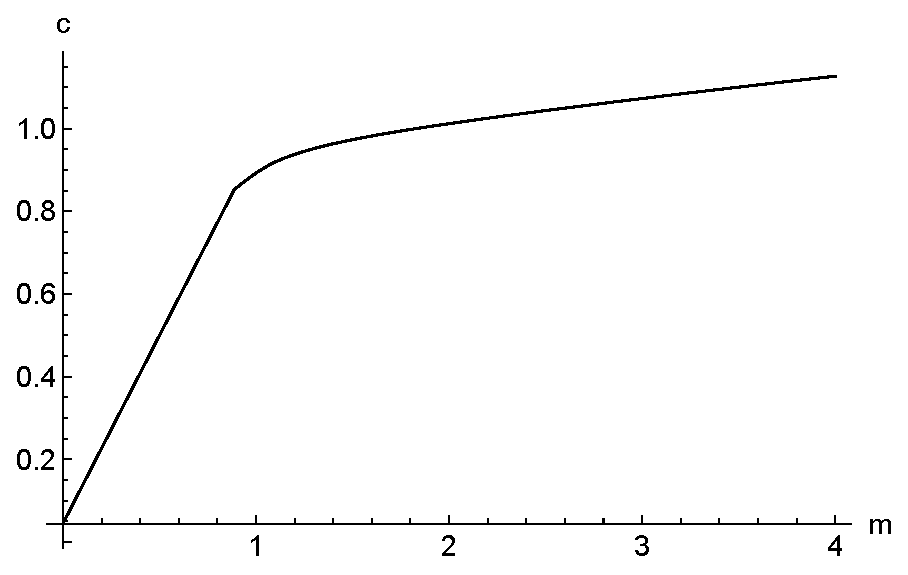
\includegraphics[width=6in]{./Figures/PlotctMultContr}
  \caption{$\cFunc_{\prdT-1}(m)$ With Portfolio Choice}
  \label{fig:PlotctMultContr}
\end{figure}

\hypertarget{PlotRiskySharetOfat}{}
\begin{figure}
  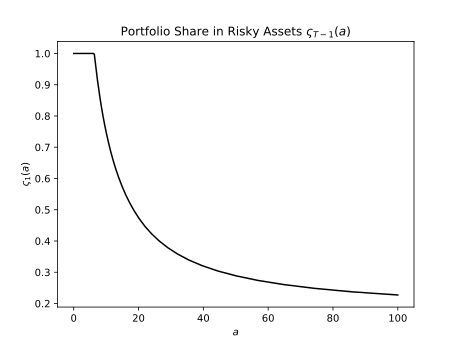
\includegraphics[width=6in]{./Figures/PlotRiskySharetOfat}
  \caption{Portfolio Share in Risky Assets $\Shr_{\prdT-1}(a)$}
  \label{fig:PlotRiskySharetOfat}
\end{figure}
